\documentclass[a4paper,14pt]{article}
\usepackage{float}
\usepackage{extsizes}
\usepackage{amsmath}
\usepackage{amssymb}
\everymath{\displaystyle}
\usepackage{geometry}
\usepackage{fancyhdr}
\usepackage{multicol}
\usepackage{graphicx}
\usepackage[brazil]{babel}
\usepackage[shortlabels]{enumitem}
\usepackage{cancel}
\columnsep=2cm
\hoffset=0cm
\textwidth=8cm
\setlength{\columnseprule}{.1pt}
\setlength{\columnsep}{2cm}
\renewcommand{\headrulewidth}{0pt}
\geometry{top=1in, bottom=1in, left=0.7in, right=0.5in}

\pagestyle{fancy}
\fancyhf{}
\fancyfoot[C]{\thepage}

\begin{document}
	
	\noindent\textbf{8FMA33~Matemática} 
	
	\begin{center}Revisão: interpretando textos e gráficos
	\end{center}
	
	\noindent\textbf{Nome:} \underline{\hspace{10cm}}
	\noindent\textbf{Data:} \underline{\hspace{4cm}}
	
	%\section*{Questões de Matemática}
	
	\begin{enumerate}
		
		\item (Enem) A tabela a seguir apresenta dados relativos a cinco países.\\
		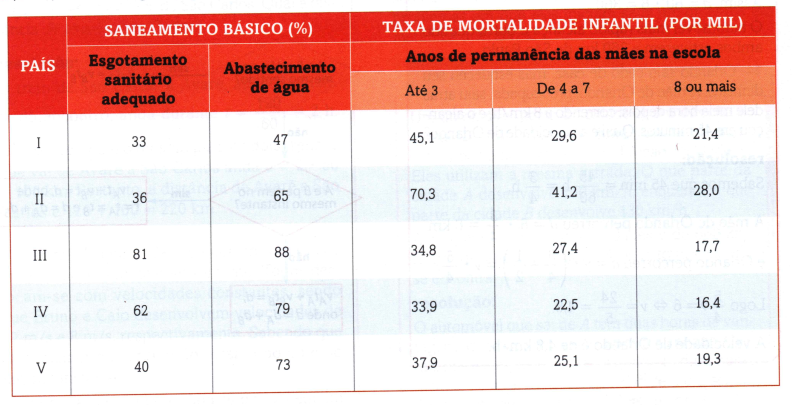
\includegraphics[width=1\linewidth]{8FMA33_imagens/imagem1}\\
		Com base nessas informações, infere-se que:
		\begin{enumerate}[a)]	
			\item a educação tem relação direta com a saúde, visto que é menor a mortalidade de filhos cujas mães possuem maior nível de escolaridade mesmo em países onde o saneamento básico é precário.
			\item o nível de escolaridade das mães tem influência na saúde dos filhos, desde que, no país em que eles residem, ou abastecimento de água favorece pelo menos 50% da população.
			\item a intensificação da educação de jovens e adultos e a ampliação do saneamento básico são medidas suficientes para se reduzir a zero a mortalidade infantil.
			\item mais crianças são acometidas pela diarreia no país III do que no país II.
			\item a taxa de mortalidade infantil é diretamente proporcional ao nível de escolaridade das mães e independe das condições sanitárias básicas. \\\\\\\\\\\\\\
		\end{enumerate}
		\begin{multicols}{2}
			\item (Enem) GH é a sigla que denomina o hormônio do crescimento (do inglês \textit{growth hormone}), indispensável para retardar o processo de envelhecimento. À medida que envelhecemos, a liberação desse hormônio na corrente sanguínea vai diminuindo. Estudos tem demonstrado porém, que alguns métodos de treinamento aumentam a produção de GH. Em uma pesquisa dez homens foram submetidos às sessões de 30 minutos de corrida, em uma esteira em diferentes intensidades: muito leve leve, moderada e máxima. As dosagens de GH, medidas por coletas de sangue feitas antes e logo após as sessões, e também 1 hora e 2 horas após o término são fornecidas no gráfico.\\
			Em qual(is) medicação(ões) a liberação de GH na corrente sanguínea em uma sessão de intensidade máxima foi maior que a liberação de GH ocorrida nas demais intensidades?\\
			\end{multicols}
		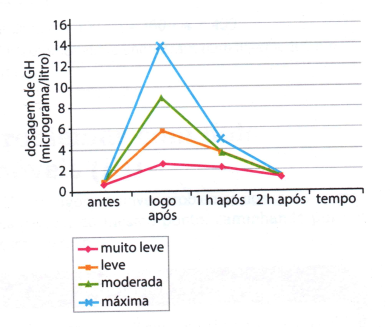
\includegraphics[width=0.7\linewidth]{8FMA33_imagens/imagem2}
		\begin{enumerate}[a)]
			\item Apenas na medicação feita logo após a sessão de treinamento.
			\item Apenas na medição feita 1 hora após a sessão de treinamento.
			\item Apenas na medicação feita 2 horas após a sessão de treinamento.
			\item Nas medições feitas logo após e 1 hora após a sessão de treinamento.
			\item Nas medições feitas logo após, 1 hora após e 2 horas após a sessão de treinamento.
			\vspace{10cm}
		\end{enumerate}

    \begin{multicols}{2}
    	\item (Enem) O gráfico mostra a variação percentual do valor do produto interno bruto (PIB) do Brasil, por trimestre, em relação ao trimestre anterior:
    	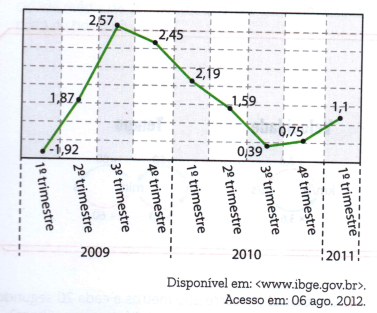
\includegraphics[width=1\linewidth]{8FMA33_imagens/imagem3}
    	De acordo com o gráfico, no período considerado o trimestre em que o Brasil teve o maior valor do PIB foi o:
    	\begin{enumerate}[a)]
    		\item Segundo trimestre de 2009.
    		\item Quarto trimestre de 2009.
    		\item Terceiro trimestre de 2010.
    		\item Quarto trimestre de 2010.
    		\item Primeiro trimestre de 2011.
    	\end{enumerate}
        \item (Enem) O sódio está presente na maioria dos alimentos industrializados podendo causar problemas cardíacos em pessoas que ingerem grandes quantidades desses alimentos. Os médicos recomendam que seus pacientes diminuam o consumo de sódio.\\
        Com base nas informações nutricionais de cinco marcas de biscoitos (A, B, C, D e E), construiu-se o gráfico, que relaciona a quantidade de sódio com porções de diferentes biscoitos.
        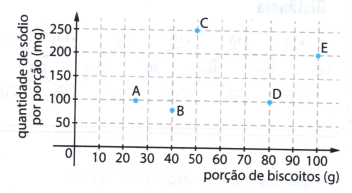
\includegraphics[width=1\linewidth]{8FMA33_imagens/imagem4}
        Qual das marcas de biscoito apresentadas tem a menor quantidade de sódio por grama do produto?
        \begin{enumerate}[a)]
        	\item $A$
        	\item $B$
        	\item $C$
        	\item $D$
        	\item $E$
        \end{enumerate}
    	\item (Enem) Um funcionário da secretaria de meio ambiente de um município resolve apresentar ao prefeito um plano de priorização para a limpeza das lagoas da cidade. Para a execução desse plano, o prefeito decide voltar suas ações, primeiramente, para aquela lagoa que tiver o maior coeficiente de impacto, o qual é definido como o produto entre o nível de contaminação médio por mercúrio em peixes e o tamanho da população ribeirinha. O quadro mostra as lagoas do município e suas correspondentes e informações.
    	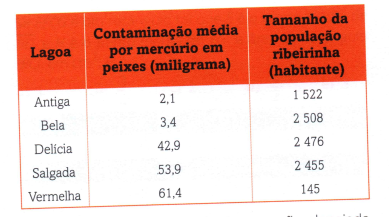
\includegraphics[width=1\linewidth]{8FMA33_imagens/imagem5}
    	 A primeira lagoa que sofrerá a intervenção planejada será a:
    	\begin{enumerate}[a)]
    		\item Antiga
    		\item Bela
    		\item Delícia
    		\item Salgada
    		\item Vermelha
    	\end{enumerate}
		\item (Enem) Doenças relacionadas ao saneamento ambiental inadequado (DRSAI) podem estar associadas ao abastecimento deficiente de água, tratamento inadequado de esgoto sanitário contaminação por resíduos sólidos ou condições precárias de moradia. O gráfico apresenta o número de casos de duas DRSAI de uma cidade:
		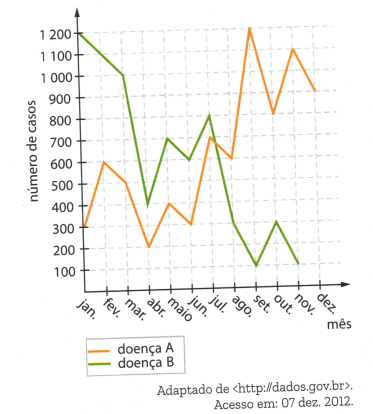
\includegraphics[width=1\linewidth]{8FMA33_imagens/imagem6}
		O mês em que se tem a maior diferença entre o número de casos das doenças de tipo A e B é:
		\begin{enumerate}[a)]
			\item Janeiro
			\item Abril
			\item Julho
			\item Setembro
			\item Novembro
		\end{enumerate}
		\item (Enem) Um comerciante abrirá um supermercado, no mês de outubro, e precisa distribuir 5 produtos de limpeza em uma gôndola de cinco prateleiras que estão dispostas uma acima da outra (um tipo de produto por prateleira). Ele sabe que a terceira prateleira oferece uma melhor visibilidade dos produtos aos clientes. Ele fez uma pesquisa sobre o número de vendas desses produtos, nos meses de Agosto e setembro, em uma loja da concorrência (mostrada a seguir), e pretende incrementar suas vendas em relação a seu concorrente, colocando na terceira prateleira de seu supermercado o produto que teve o maior índice de aumento nas vendas do mês de setembro em relação ao mês de agosto, na loja concorrente.
		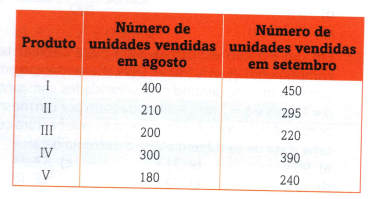
\includegraphics[width=1\linewidth]{8FMA33_imagens/imagem7}
		O comerciante deve colocar na terceira prateleira o produto número.
		\begin{enumerate}[a)]
			\item I
			\item II
			\item III
			\item IV
			\item V
		\end{enumerate}
		\item (Enem) Um país decide investir recursos na educação em suas cidades que tenham um alto nível de analfabetismo os recursos serão divididos de acordo com a idade média da população que é analfabeta, conforme apresentado no quadro.
		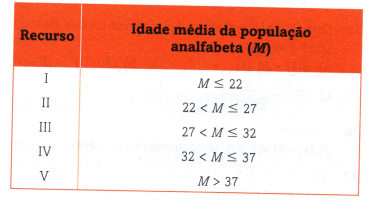
\includegraphics[width=1\linewidth]{8FMA33_imagens/imagem8}
		Uma cidade desse país possui $\frac{60}{100}$ \\\\do total de analfabetos e sua população composto por mulheres.
\\
		A média de idade das mulheres analfabetas é de 30 anos, e a média de idade dos homens analfabetos é de 35 anos.
\\
		Considerando a média de idade da população analfabeta dessa cidade, ela receberá o recurso:
		\begin{enumerate}[a)]
			\item I
			\item II
			\item III
			\item IV
			\item V
		\end{enumerate}
	$~$ \\ $~$ \\ $~$ \\ $~$ \\ $~$ \\ $~$ \\ $~$ \\ $~$ \\ $~$ \\ $~$ \\ $~$ \\ $~$ \\ $~$ \\ $~$ \\ $~$ \\ $~$ \\ $~$ \\ $~$ \\ $~$ \\ $~$ \\ $~$ \\ $~$ \\$~$ \\ $~$ \\ $~$ \\ $~$ \\ $~$ \\ $~$ \\ $~$ \\ $~$ \\ $~$ \\ $~$ \\ $~$ \\ $~$ \\ $~$ \\ $~$ \\ $~$ \\ $~$ \\ $~$ \\ $~$ \\ $~$ \\ $~$ \\ $~$ \\ $~$ \\$~$ \\ $~$ \\ $~$ \\ $~$ \\ $~$ \\ $~$ \\ $~$
    \end{multicols}
	\end{enumerate}
\end{document}